Fixed points and (known) conserved quantites for the concentric, axis-parallel (CAP) families of \cref{sec:03-other-conc} appear in
\cref{tab:n3-conc-families}. Those for the non-concentric (NCAP) families of \cref{sec:03-non-conc} appear in
\cref{tab:n3-non-conc-families}. A diagram appears in \cref{fig:03-transformations} which illustrate how certain pairs of families are interrelated by either similarity or polar transformations.

\begin{table}
\centering
\begin{tabular}{|r|c|c|l|}
\hline
Family & Fixed & Conserves & Notes \\
\hline
Confocal & $X_9$ & $L$, $J$, $r/R$, $\sum\cos\theta_i$ & i.e., billiard 3-periodics \\
\hline
Incircle & $X_1$ & $R$, $\sum\cos\theta_i$ & \makecell[lc]{sum of cosines same as\\confocal affine pre-image} \\
\hline
Circumcircle & $X_3$ & \makecell[cc]{$\sum{s_i^2}$, $\prod\cos\theta_i$,\\$r_h$,$R_h$} & \makecell[lc]{product of cosines same as\\excentrals' in confocal affine\\pre-image} \\
\hline
\makecell[rc]{Confocal\\Excentrals} & $X_6$ & \makecell[cc]{$A'/A$, $\prod\cos\theta_i'$,\\$\sum{(s_i')^2}/\prod{s_i'}$} & \makecell[lc]{primed quantities refer to those\\of the excentral family}  \\
\hline
Homothetic & $X_2$ & $A$, $\sum{s_i^2}$, $\omega$, $\sum\cot\theta_i$ & affine image of concentric circles  \\
\hline
Dual & $X_4$ & n/a &  \\
\hline
\end{tabular}
\caption{Summary of fixed points and (known) conserved quantites for the concentric, axis-parallel (CAP) families mentioned in \cref{sec:03-other-conc}.}
\label{tab:n3-conc-families}
\end{table}

\begin{table}
\centering
\begin{tabular}{|r|c|c|l|}
\hline
Family & Fixed & Conserves & Notes \\
\hline
\makecell[rc]{Poristic\\(bicentric)} & $X_1$, $X_3$, $X_{40}$, $\ldots$ & $\sum\cos\theta_i,a_9/b_9$ & \makecell[lc]{polar image of Confocal family\\wrt to a focus} \\
\hline
\makecell[rt]{Poristic\\Excentrals} & $X_2$, $X_3$, $X_4$, $X_5$ & $\sum{s_i^2}$, $\prod\cos\theta_i$ & \makecell[lt]{Inscribed in circle;\\caustic is MacBeath inconic} \\
\hline
Brocard & \makecell[lc]{$X_3$, $X_6$, $X_{15}$, $X_{16}$,\\$X_{39}$, $X_{182},\ldots$,\\$\Omega_1$, $\Omega_2$} & $\sum{s_i^{-2}}$, $\omega$, $\sum\cot\theta_i$ & \makecell[lc]{polar image of Homothetic\\family wrt caustic focus;\\inscribed in circle;\\caustic is Brocard inellipse}\\
%\hline
%focus-Inversive & $X_7$ & $L,\sum\cos\theta_i$ & \makecell[lc]{inversive image of Confocals\\wrt a focus; non-Ponceletian;\\inscribed in Pascal's limaçon;\\caustic non-ellipse}\\
\hline
\end{tabular}
\caption{Summary of fixed points and (known) conserved quantites for the non-concentric, axis-parallel (NCAP) families of \cref{sec:03-non-conc}.}
\label{tab:n3-non-conc-families}
\end{table}



\begin{figure}
    \centering
    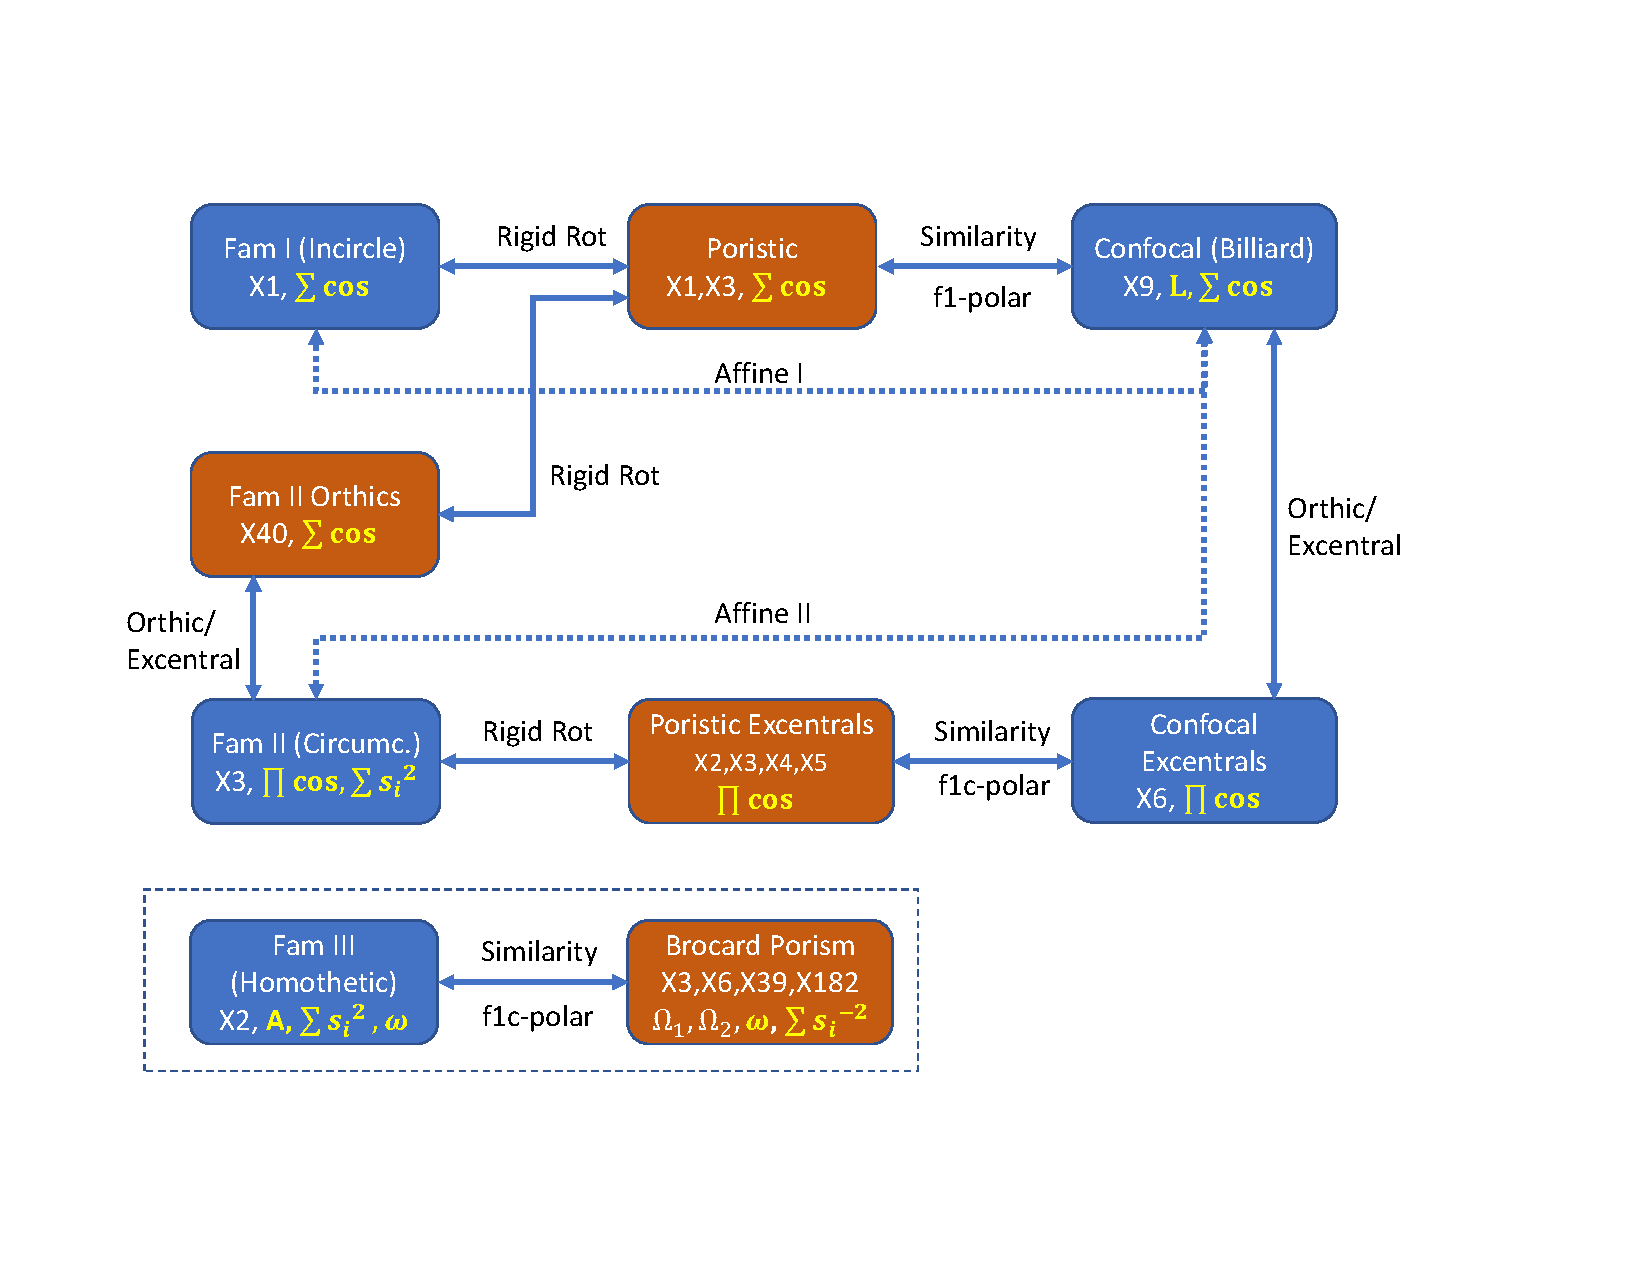
\includegraphics[width=\textwidth]{chap_03/pics/pics_03_250_poncelet_transformations.pdf}
  \caption{Families mentioned in this chapter (blue ones are concentric, tan ones are non-concentric), as well as the transformations under which certain families are interrelated.}
    \label{fig:03-transformations}
\end{figure}